\subsection{Sphere-geodesic-line picking}
\label{sec:sphere_geodesic_line}


Sphere-geodesic-line picking is similar to sphere-line picking, except
that the ``lines'' are geodesics on the surface of the sphere, and the
distance metric is the length of these lines.

Figures ...

\begin{figure}[tbp]
  \begin{center}
    \subfloat[\label{fig:sphere_geo_eg}
    Example.]{\includegraphics[width=0.4\columnwidth]{../Matlab/Plots/LinePicking_test_sim_sphere_geodesic_eg.eps}} 
    \hspace{6mm}
    \subfloat[\label{fig:sphere_geo_pdf}PDF.]{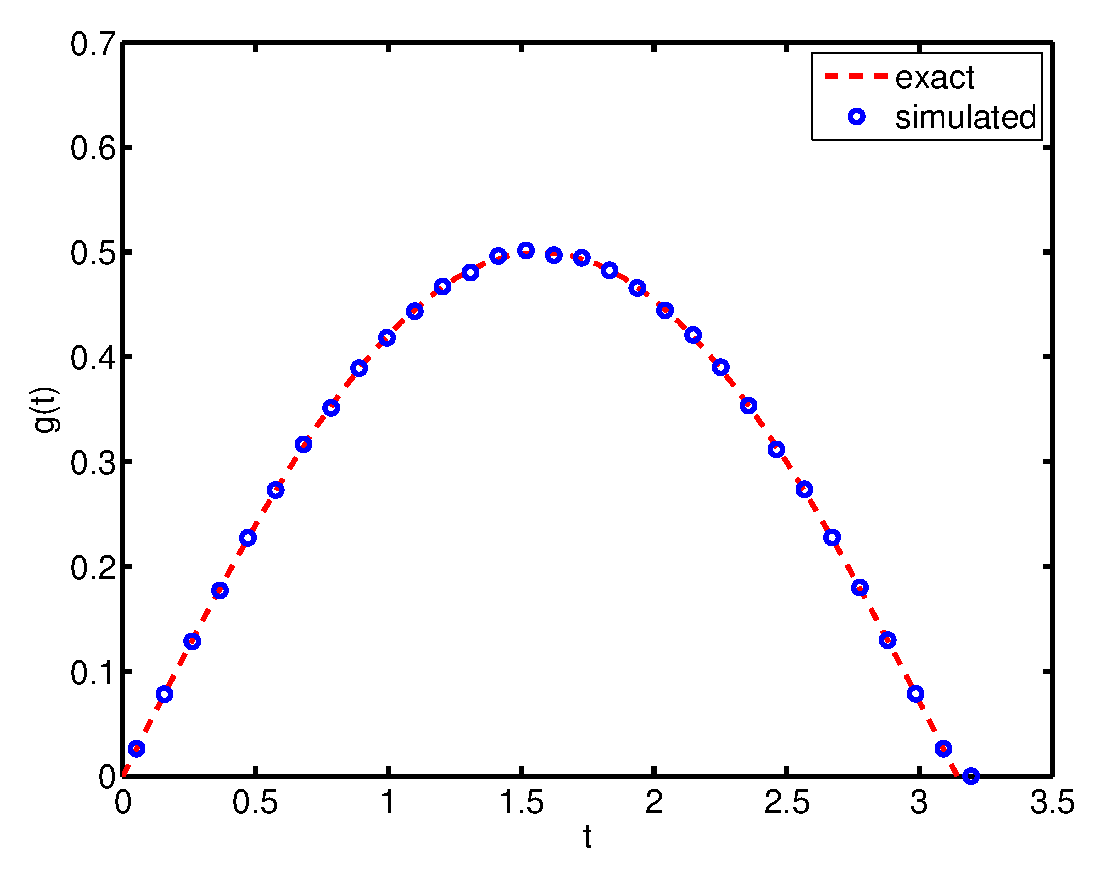
\includegraphics[width=0.48\columnwidth]{../Matlab/Plots/LinePicking_test_sim_sphere_geodesic.eps}}
    \caption{The sphere-geodesic-line picking problem.}
  \end{center} 
\vspace{-4mm}
\end{figure}

\subsubsection{PDF}


\subsubsection{CDF}


\subsubsection{Moments}



